\documentclass[a4paper]{report}
% Some basic packages
\usepackage[utf8]{inputenc}
\usepackage[T1]{fontenc}
\usepackage{textcomp}
\usepackage[english]{babel}
\usepackage{url}
\usepackage{graphicx}
\usepackage{float}
\usepackage{booktabs}
\usepackage{enumitem}

\pdfminorversion=7

% Don't indent paragraphs, leave some space between them
\usepackage{parskip}

% Hide page number when page is empty
\usepackage{emptypage}
\usepackage{subcaption}
\usepackage{multicol}
\usepackage{xcolor}

% Other font I sometimes use.
% \usepackage{cmbright}

% Math stuff
\usepackage{amsmath, amsfonts, mathtools, amsthm, amssymb}
% Fancy script capitals
\usepackage{mathrsfs}
\usepackage{cancel}
% Bold math
\usepackage{bm}
% Some shortcuts
\newcommand\N{\ensuremath{\mathbb{N}}}
\newcommand\R{\ensuremath{\mathbb{R}}}
\newcommand\Z{\ensuremath{\mathbb{Z}}}
\renewcommand\O{\ensuremath{\emptyset}}
\newcommand\Q{\ensuremath{\mathbb{Q}}}
\newcommand\C{\ensuremath{\mathbb{C}}}
\renewcommand\L{\ensuremath{\mathcal{L}}}

% Package for Petri Net drawing
\usepackage[version=0.96]{pgf}
\usepackage{tikz}
\usetikzlibrary{arrows,shapes,automata,petri}
\usepackage{tikzit}
\input{petri_nets_style.tikzstyles}

% Easily typeset systems of equations (French package)
\usepackage{systeme}

% Put x \to \infty below \lim
\let\svlim\lim\def\lim{\svlim\limits}

%Make implies and impliedby shorter
\let\implies\Rightarrow
\let\impliedby\Leftarrow
\let\iff\Leftrightarrow
\let\epsilon\varepsilon

% Add \contra symbol to denote contradiction
\usepackage{stmaryrd} % for \lightning
\newcommand\contra{\scalebox{1.5}{$\lightning$}}

% \let\phi\varphi

% Command for short corrections
% Usage: 1+1=\correct{3}{2}

\definecolor{correct}{HTML}{009900}
\newcommand\correct[2]{\ensuremath{\:}{\color{red}{#1}}\ensuremath{\to }{\color{correct}{#2}}\ensuremath{\:}}
\newcommand\green[1]{{\color{correct}{#1}}}

% horizontal rule
\newcommand\hr{
    \noindent\rule[0.5ex]{\linewidth}{0.5pt}
}

% hide parts
\newcommand\hide[1]{}

% si unitx
\usepackage{siunitx}
\sisetup{locale = FR}

% Environments
\makeatother
% For box around Definition, Theorem, \ldots
\usepackage{mdframed}
\mdfsetup{skipabove=1em,skipbelow=0em}
\theoremstyle{definition}
\newmdtheoremenv[nobreak=true]{definitie}{Definitie}
\newmdtheoremenv[nobreak=true]{eigenschap}{Eigenschap}
\newmdtheoremenv[nobreak=true]{gevolg}{Gevolg}
\newmdtheoremenv[nobreak=true]{lemma}{Lemma}
\newmdtheoremenv[nobreak=true]{propositie}{Propositie}
\newmdtheoremenv[nobreak=true]{stelling}{Stelling}
\newmdtheoremenv[nobreak=true]{wet}{Wet}
\newmdtheoremenv[nobreak=true]{postulaat}{Postulaat}
\newmdtheoremenv{conclusie}{Conclusie}
\newmdtheoremenv{toemaatje}{Toemaatje}
\newmdtheoremenv{vermoeden}{Vermoeden}
\newtheorem*{herhaling}{Herhaling}
\newtheorem*{intermezzo}{Intermezzo}
\newtheorem*{notatie}{Notatie}
\newtheorem*{observatie}{Observatie}
\newtheorem*{exe}{Exercise}
\newtheorem*{opmerking}{Opmerking}
\newtheorem*{praktisch}{Praktisch}
\newtheorem*{probleem}{Probleem}
\newtheorem*{terminologie}{Terminologie}
\newtheorem*{toepassing}{Toepassing}
\newtheorem*{uovt}{UOVT}
\newtheorem*{vb}{Voorbeeld}
\newtheorem*{vraag}{Vraag}

\newmdtheoremenv[nobreak=true]{definition}{Definition}
\newtheorem*{eg}{Example}
\newtheorem*{notation}{Notation}
\newtheorem*{previouslyseen}{As previously seen}
\newtheorem*{remark}{Remark}
\newtheorem*{note}{Note}
\newtheorem*{problem}{Problem}
\newtheorem*{observe}{Observe}
\newtheorem*{property}{Property}
\newtheorem*{intuition}{Intuition}
\newmdtheoremenv[nobreak=true]{prop}{Proposition}
\newmdtheoremenv[nobreak=true]{theorem}{Theorem}
\newmdtheoremenv[nobreak=true]{corollary}{Corollary}

% End example and intermezzo environments with a small diamond (just like proof
% environments end with a small square)
\usepackage{etoolbox}
\AtEndEnvironment{vb}{\null\hfill$\diamond$}%
\AtEndEnvironment{intermezzo}{\null\hfill$\diamond$}%
% \AtEndEnvironment{opmerking}{\null\hfill$\diamond$}%

% Fix some spacing
% http://tex.stackexchange.com/questions/22119/how-can-i-change-the-spacing-before-theorems-with-amsthm
\makeatletter
\def\thm@space@setup{%
  \thm@preskip=\parskip \thm@postskip=0pt
}


% Exercise 
% Usage:
% \exercise{5}
% \subexercise{1}
% \subexercise{2}
% \subexercise{3}
% gives
% Exercise 5
%   Exercise 5.1
%   Exercise 5.2
%   Exercise 5.3
\newcommand{\exercise}[1]{%
    \def\@exercise{#1}%
    \subsection*{Exercise #1}
}

\newcommand{\subexercise}[1]{%
    \subsubsection*{Exercise \@exercise.#1}
}


% \lecture starts a new lecture (les in dutch)
%
% Usage:
% \lecture{1}{di 12 feb 2019 16:00}{Inleiding}
%
% This adds a section heading with the number / title of the lecture and a
% margin paragraph with the date.

% I use \dateparts here to hide the year (2019). This way, I can easily parse
% the date of each lecture unambiguously while still having a human-friendly
% short format printed to the pdf.

\usepackage{xifthen}
\def\testdateparts#1{\dateparts#1\relax}
\def\dateparts#1 #2 #3 #4 #5\relax{
    \marginpar{\small\textsf{\mbox{#1 #2 #3 #5}}}
}

\def\@lecture{}%
\newcommand{\lecture}[3]{
    \ifthenelse{\isempty{#3}}{%
        \def\@lecture{Lecture #1}%
    }{%
        \def\@lecture{Lecture #1: #3}%
    }%
    \subsection*{\@lecture}
    \marginpar{\small\textsf{\mbox{#2}}}
}



% These are the fancy headers
\usepackage{fancyhdr}
\pagestyle{fancy}

% LE: left even
% RO: right odd
% CE, CO: center even, center odd
% My name for when I print my lecture notes to use for an open book exam.
% \fancyhead[LE,RO]{Gilles Castel}

\fancyhead[RO,LE]{\@lecture} % Right odd,  Left even
\fancyhead[RE,LO]{}          % Right even, Left odd

\fancyfoot[RO,LE]{\thepage}  % Right odd,  Left even
\fancyfoot[RE,LO]{}          % Right even, Left odd
\fancyfoot[C]{\leftmark}     % Center

\makeatother




% Todonotes and inline notes in fancy boxes
\usepackage{todonotes}
\usepackage{tcolorbox}

% Make boxes breakable
\tcbuselibrary{breakable}

% Verbetering is correction in Dutch
% Usage: 
% \begin{verbetering}
%     Lorem ipsum dolor sit amet, consetetur sadipscing elitr, sed diam nonumy eirmod
%     tempor invidunt ut labore et dolore magna aliquyam erat, sed diam voluptua. At
%     vero eos et accusam et justo duo dolores et ea rebum. Stet clita kasd gubergren,
%     no sea takimata sanctus est Lorem ipsum dolor sit amet.
% \end{verbetering}
\newenvironment{verbetering}{\begin{tcolorbox}[
    arc=0mm,
    colback=white,
    colframe=green!60!black,
    title=Opmerking,
    fonttitle=\sffamily,
    breakable
]}{\end{tcolorbox}}

% Noot is note in Dutch. Same as 'verbetering' but color of box is different
\newenvironment{noot}[1]{\begin{tcolorbox}[
    arc=0mm,
    colback=white,
    colframe=white!60!black,
    title=#1,
    fonttitle=\sffamily,
    breakable
]}{\end{tcolorbox}}




% Figure support as explained in my blog post.
\usepackage{import}
\usepackage{xifthen}
\usepackage{pdfpages}
\usepackage{transparent}
\newcommand{\incfig}[1]{%
    \def\svgwidth{\columnwidth}
    \import{./figures/}{#1.pdf_tex}
}

% Fix some stuff
% %http://tex.stackexchange.com/questions/76273/multiple-pdfs-with-page-group-included-in-a-single-page-warning
\pdfsuppresswarningpagegroup=1


% My name
\author{Bruno M. Pacheco}

 
\begin{document}
 
\title{Relatório 2}
\author{Bruno M. Pacheco\\
DAS 5142 - Sistemas Dinâmicos}
 
\maketitle
 
\exercise{}

\subsubsection*{a)}

Para o primeiro sistema, podemos encontrar os pontos de equilíbrio igualando $\bm{\dot{x}}$ a zero, ou seja
\begin{align*}
    \dot{x}_1 = 0 \implies \overline{x}_1 = \pm\sqrt{\mu} \\
    \dot{x}_2 = 0 \implies \overline{x}_2 = 0 \\
\end{align*}
, assim, os pontos do equilíbrio do sistema dependem do parâmetro $\mu$ e têm forma $(\pm\sqrt{\mu} ,0)$. Como não consideramos soluções imaginárias, o sistema só possui equilíbrio para $\mu\ge 0$.

Em relação à estabilidade no ponto de equilíbrio, temos que a matriz jacobiana do sistema é \[
    \begin{bmatrix} -2x_1 & 0 \\ 0 & -1  \end{bmatrix} 
\] e possui autovalores $-1$ e $\pm 2\sqrt{\mu}$. Assim, concluímos que o ramo superior dos pontos de equilíbrio, aquele da forma $\sqrt{\mu}$ é estável, enquanto o ramo inferior, de forma $-\sqrt{\mu}$ é instável e um ponto de sela.

Para $\mu = 0$, temos um autovalor no semiplano esquerdo e um autovalor nulo, o que nos indica que esta é uma bifurcação sela-nó.

\subsubsection*{b)}

Podemos observar o comportamento dos ramos do ponto de equilíbrio na figura \ref{fig:figures-lab2_1_pitchfork-pdf}.

\begin{figure}[H]
    \centering
    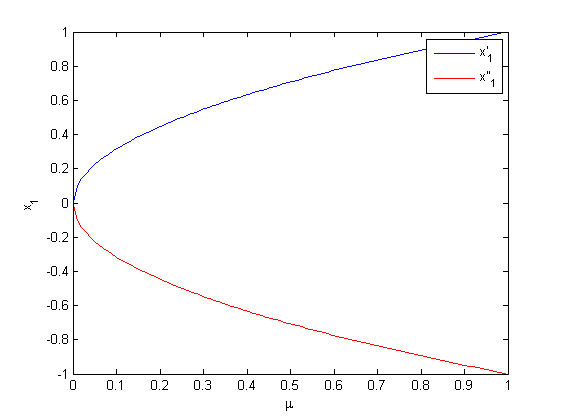
\includegraphics[width=0.6\textwidth]{figures/lab2_1_pitchfork.png}
    \caption{Diagrama de variação dos equilíbrios do sistema 1 em função do parâmetro $\mu$. Em azul, o ramo estável e em vermelho o ramo instável.}

    \label{fig:figures-lab2_1_pitchfork-pdf}
\end{figure}

\subsubsection*{c)}

Utilizando o aplicativo \emph{pplane8}, simulou-se o sistema para 3 combinações do parâmetro $\mu$. Os resultados podem ser observados na figura \ref{fig:pplane-1}.

\begin{figure}[H]
    \centering
    \begin{subfigure}{0.29\textwidth}
	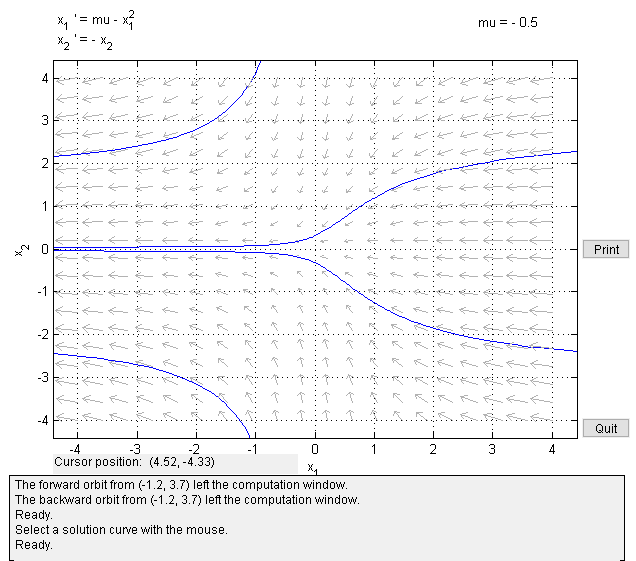
\includegraphics[width=\textwidth]{figures/lab2_1_pplane_inst.png}
	\caption{$\mu=-0,5$}
    \end{subfigure}
    \begin{subfigure}{0.29\textwidth}
	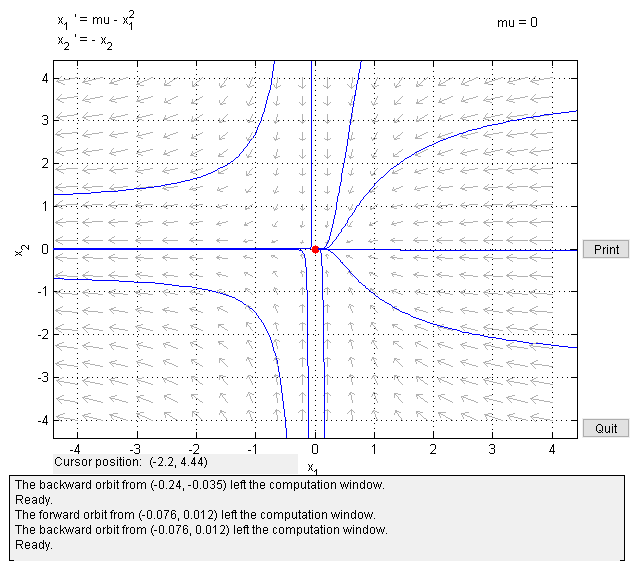
\includegraphics[width=\textwidth]{figures/lab2_1_pplane_0.png}
	\caption{$\mu=0$}
    \end{subfigure}
    \begin{subfigure}{0.29\textwidth}
	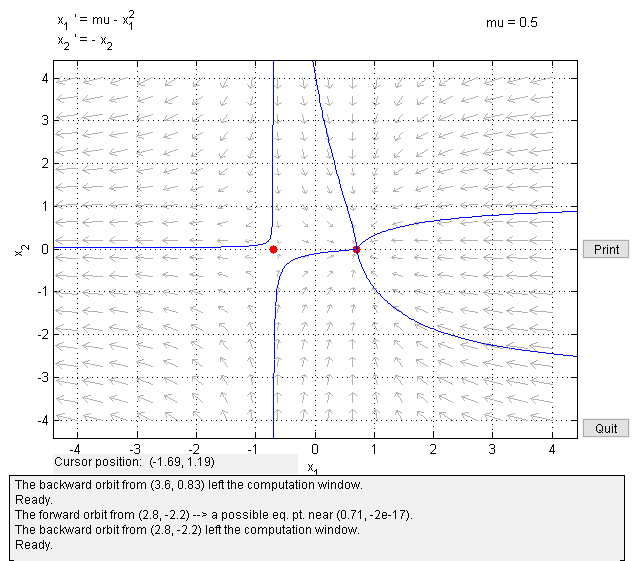
\includegraphics[width=\textwidth]{figures/lab2_1_pplane_st.png}
	\caption{$\mu=0,5$}
    \end{subfigure}
    \caption{Espaço de estados do modelo do primeiro sistema para diferentes parâmetros. Pontos de equilíbrio são representados por pontos vermelhos e as trajetórias dos estados são os traços azuis.}
    \label{fig:pplane-1}
\end{figure}

\exercise{}

\subsubsection*{a)}

Para o segundo sistema, identificou-se duas possíveis formas para o ponto de equilíbrio:
\begin{align*}
    \bm{\overline{x}}_1 &= \begin{bmatrix} 0 \\ 0 \end{bmatrix} \\
    \bm{\overline{x}}_2 &= \begin{bmatrix} \mu \\ 0 \end{bmatrix} 
.\end{align*}

Para determinar a estabilidade, analisamos a jacobiana do sistema, ou seja, a matriz \[
    \begin{bmatrix} \mu-2x_1 & 0 \\ 0 & -1 \end{bmatrix} 
\]. Temos que, para os pontos $\bm{\overline{x}}_1$, a matriz possui autovalores \[
\bm{\lambda} = \begin{bmatrix}   -1 \\ \mu \end{bmatrix}
\] sendo, portanto, estável somente para $\mu<0$. Agora para os pontos $\bm{\overline{x}}_2$, os autovalores são \[
\bm{\lambda} = \begin{bmatrix}   -1 \\ -\mu \end{bmatrix}
\], o que nos indica que esses pontos são estáveis somente para $\mu>0$.

Para o caso de $\mu=0$, têm-se um autovalor nulo, portanto não podemos concluir nada.

\subsubsection*{b)}

Pode-se observar o comportamento dos ramos do ponto de equilíbrio na figura \ref{fig:figures-lab2_2_pitchfork-png}.

\begin{figure}[H]
    \centering
    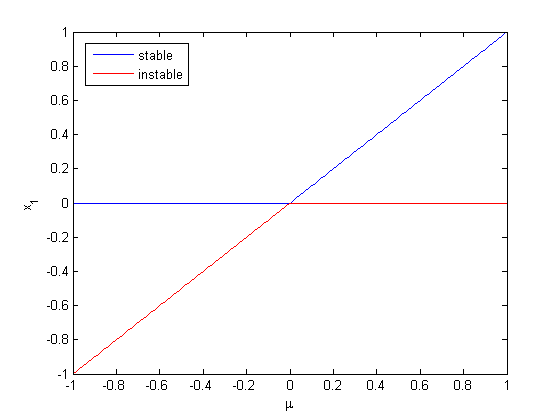
\includegraphics[width=0.6\textwidth]{figures/lab2_2_pitchfork.png}
    \caption{Diagrama de variação dos equilíbrios do sistema 2 em função do parâmetro $\mu$. Em azul, o ramo estável e em vermelho o ramo instável.}
    \label{fig:figures-lab2_2_pitchfork-png}
\end{figure}

\subsubsection*{c)}

As simulações através do aplicativo \emph{pplane8} podem ser observadas na figura \ref{fig:pplane-2}. Verifica-se o encontrado de forma analítica.

\begin{figure}[H]
    \centering
    \begin{subfigure}{0.29\textwidth}
	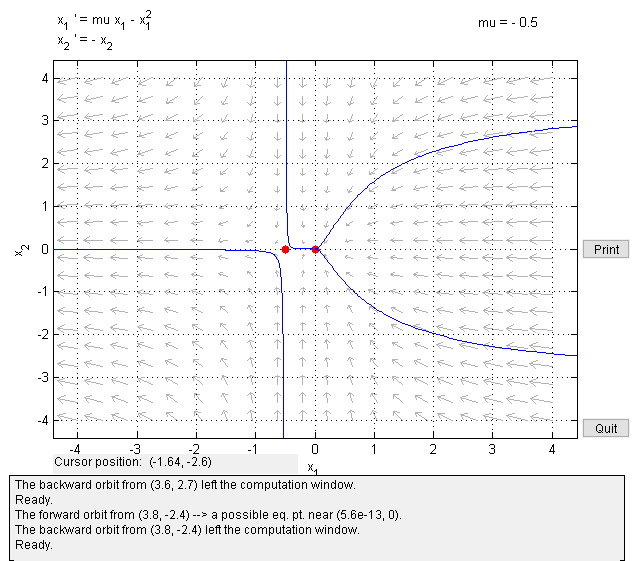
\includegraphics[width=\textwidth]{figures/lab2_2_pplane_neg.png}
	\caption{$\mu=-0,5$}
    \end{subfigure}
    \begin{subfigure}{0.29\textwidth}
	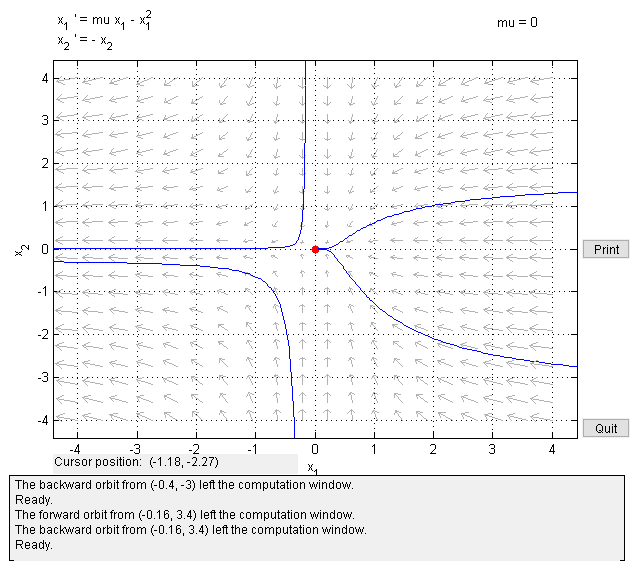
\includegraphics[width=\textwidth]{figures/lab2_2_pplane_0.png}
	\caption{$\mu=0$}
    \end{subfigure}
    \begin{subfigure}{0.29\textwidth}
	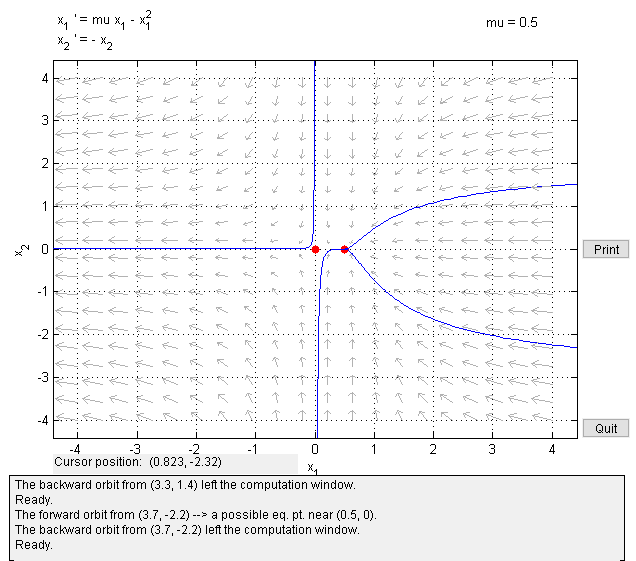
\includegraphics[width=\textwidth]{figures/lab2_2_pplane_pos.png}
	\caption{$\mu=0,5$}
    \end{subfigure}
    \caption{Espaço de estados do modelo do segundo sistema para diferentes parâmetros. Pontos de equilíbrio são representados por pontos vermelhos e as trajetórias dos estados são os traços azuis.}
    \label{fig:pplane-2}
\end{figure}

\exercise{}

\subsubsection*{a)}

Para o terceiro sistema, os pontos de equilíbrio têm três possíveis formas:
\begin{align*}
    \bm{\overline{x}}_1 &= \begin{bmatrix} \sqrt{\mu} \\ 0 \end{bmatrix} \\
    \bm{\overline{x}}_2 &= \begin{bmatrix} -\sqrt{\mu} \\ 0 \end{bmatrix} \\
    \bm{\overline{x}}_3 &= \begin{bmatrix} 0 \\ 0 \end{bmatrix} \\
.\end{align*}
Nota-se que os dois primeiros só são válidos para $\mu>0$, uma vez que pontos de equilíbrio complexos não são válidos.

A estabilidade desses pode ser determinada através da matriz jacobiana \[
    \begin{bmatrix} \mu-3x_1^2 & 0 \\ 0 & -1 \end{bmatrix} 
\]. Os respectivos autovalores são
\begin{align*}
    \bm{\lambda}_1 &= \begin{bmatrix}   -1 \\ -2\mu \end{bmatrix} \\
    \bm{\lambda}_2 &= \begin{bmatrix}   -1 \\ -2\mu \end{bmatrix} \\
    \bm{\lambda}_3 &= \begin{bmatrix}   -1 \\ \mu \end{bmatrix} \\
.\end{align*}
Concluímos, então, que os ramos referentes a $\bm{\overline{x}}_1$ e $\bm{\overline{x}}_2$ são estáveis para $\mu>0$, enquanto o ramo associado a $\bm{\overline{x}}_3$ é estável para $\mu<0$, o que resulta em uma bifurcação do tipo tridente supercrítica.

\subsubsection*{b)}

O diagrama de variação dos equilíbrio pode ser observado na figura \ref{fig:figures-lab2_3_pitchfork-png}.

\begin{figure}[H]
    \centering
    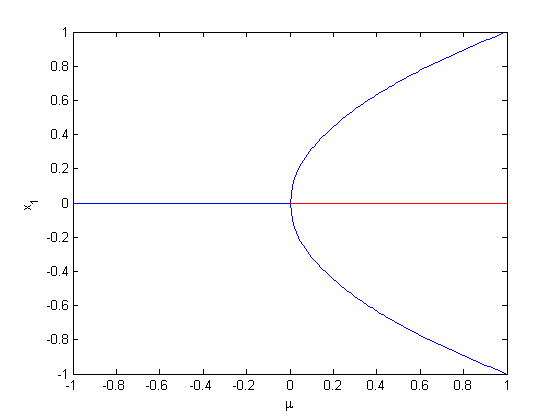
\includegraphics[width=0.6\textwidth]{figures/lab2_3_pitchfork.png}
    \caption{Diagrama de variação dos equilíbrios do sistema 3 em função do parâmetro $\mu$. Em azul, o ramo estável e em vermelho o ramo instável.}
    \label{fig:figures-lab2_3_pitchfork-png}
\end{figure}

\subsubsection*{c)}

A simulação do sistema no aplicativo \emph{pplane8} pode ser observado na figura \ref{fig:pplane-3}.

\begin{figure}[H]
    \centering
    \begin{subfigure}{0.29\textwidth}
	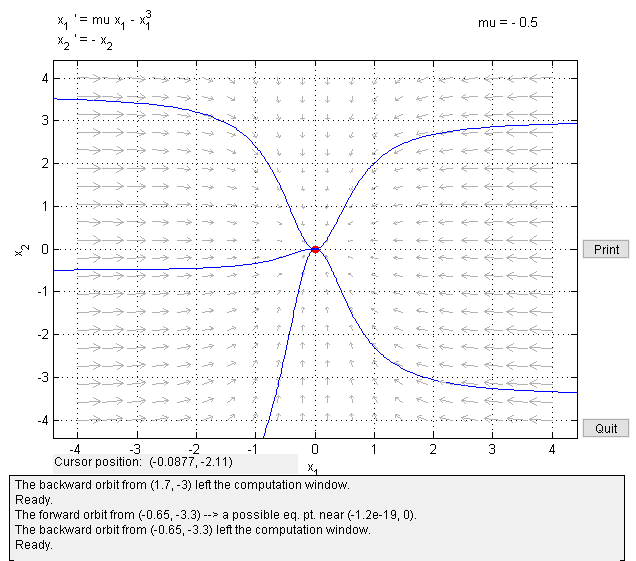
\includegraphics[width=\textwidth]{figures/lab2_3_pplane_neg.png}
	\caption{$\mu=-0,5$}
    \end{subfigure}
    \begin{subfigure}{0.29\textwidth}
	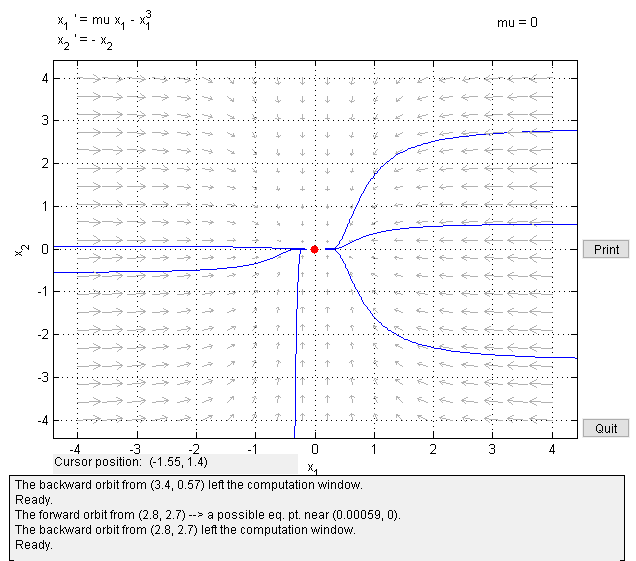
\includegraphics[width=\textwidth]{figures/lab2_3_pplane_0.png}
	\caption{$\mu=0$}
    \end{subfigure}
    \begin{subfigure}{0.29\textwidth}
	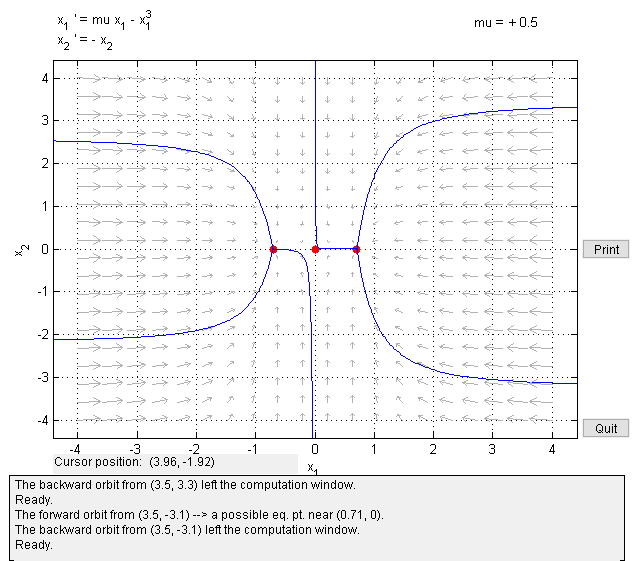
\includegraphics[width=\textwidth]{figures/lab2_3_pplane_pos.png}
	\caption{$\mu=0,5$}
    \end{subfigure}
    \caption{Espaço de estados do modelo do terceiro sistema para diferentes parâmetros. Pontos de equilíbrio são representados por pontos vermelhos e as trajetórias dos estados são os traços azuis.}
    \label{fig:pplane-3}
\end{figure}

\exercise{}

\subsubsection*{a)}

Para o sistema 4, os pontos de equilíbrio têm três possíveis formas:
\begin{align*}
    \bm{\overline{x}}_1 &= \begin{bmatrix} \sqrt{-\mu} \\ 0 \end{bmatrix} \\
    \bm{\overline{x}}_2 &= \begin{bmatrix} -\sqrt{-\mu} \\ 0 \end{bmatrix} \\
    \bm{\overline{x}}_3 &= \begin{bmatrix} 0 \\ 0 \end{bmatrix} \\
.\end{align*}
Nota-se que os dois primeiros só são válidos para $\mu<0$, uma vez que pontos de equilíbrio complexos não são válidos.

A estabilidade desses pode ser determinada através da matriz jacobiana \[
    \begin{bmatrix} \mu+3x_1^2 & 0 \\ 0 & -1 \end{bmatrix} 
\]. Os respectivos autovalores são
\begin{align*}
    \bm{\lambda}_1 &= \begin{bmatrix}   -1 \\ -2\mu \end{bmatrix} \\
    \bm{\lambda}_2 &= \begin{bmatrix}   -1 \\ -2\mu \end{bmatrix} \\
    \bm{\lambda}_3 &= \begin{bmatrix}   -1 \\ \mu \end{bmatrix} \\
.\end{align*}
Concluímos, então, que os ramos referentes a $\bm{\overline{x}}_1$ e $\bm{\overline{x}}_2$ são instáveis enquanto o ramo associado a $\bm{\overline{x}}_3$ é estável para $\mu<0$, o que resulta em uma bifurcação subcrítica.

\subsubsection*{b)}

O diagrama de variação dos equilíbrio pode ser observado na figura \ref{fig:figures-lab2_4_pitchfork-png}.

\begin{figure}[H]
    \centering
    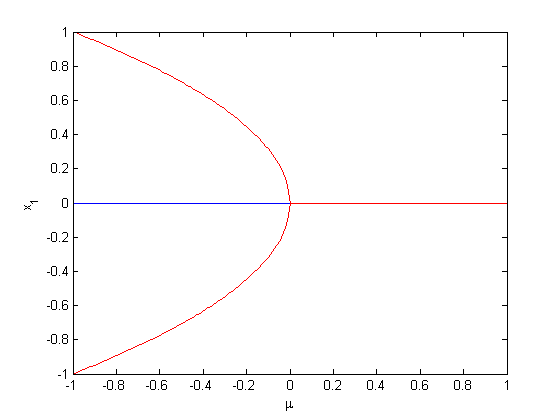
\includegraphics[width=0.6\textwidth]{figures/lab2_4_pitchfork.png}
    \caption{Diagrama de variação dos equilíbrios do sistema 4 em função do parâmetro $\mu$. Em azul, o ramo estável e em vermelho o ramo instável.}
    \label{fig:figures-lab2_4_pitchfork-png}
\end{figure}

\subsubsection*{c)}

A simulação do sistema no aplicativo \emph{pplane8} pode ser observado na figura \ref{fig:pplane-4}.

\begin{figure}[H]
    \centering
    \begin{subfigure}{0.29\textwidth}
	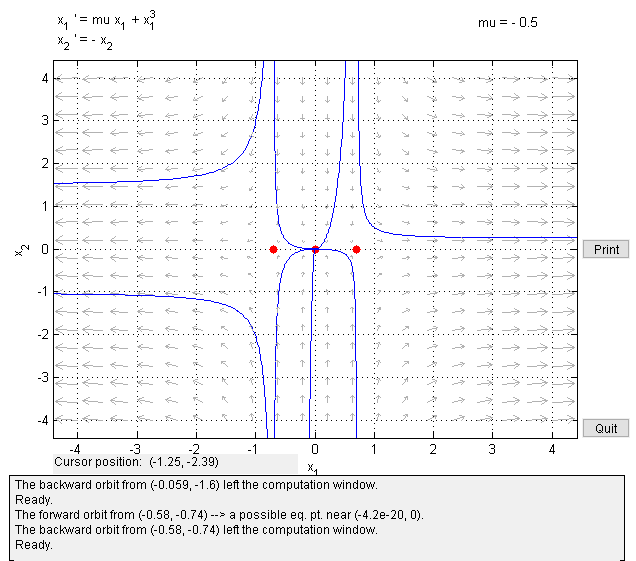
\includegraphics[width=\textwidth]{figures/lab2_4_pplane_neg.png}
	\caption{$\mu=-0,5$}
    \end{subfigure}
    \begin{subfigure}{0.29\textwidth}
	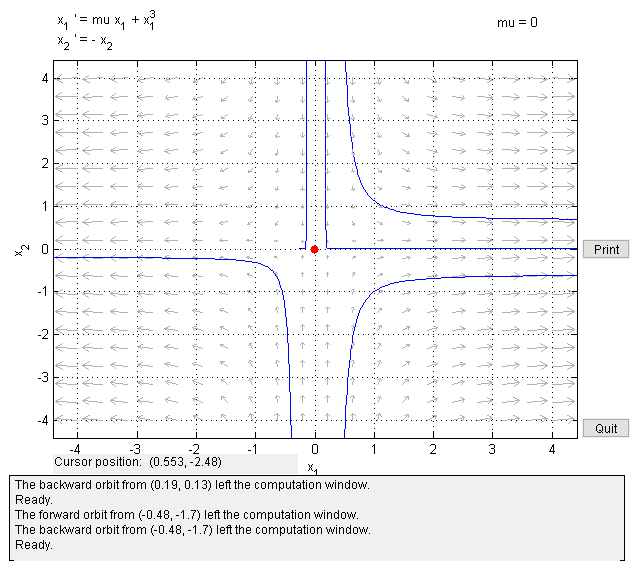
\includegraphics[width=\textwidth]{figures/lab2_4_pplane_0.png}
	\caption{$\mu=0$}
    \end{subfigure}
    \begin{subfigure}{0.29\textwidth}
	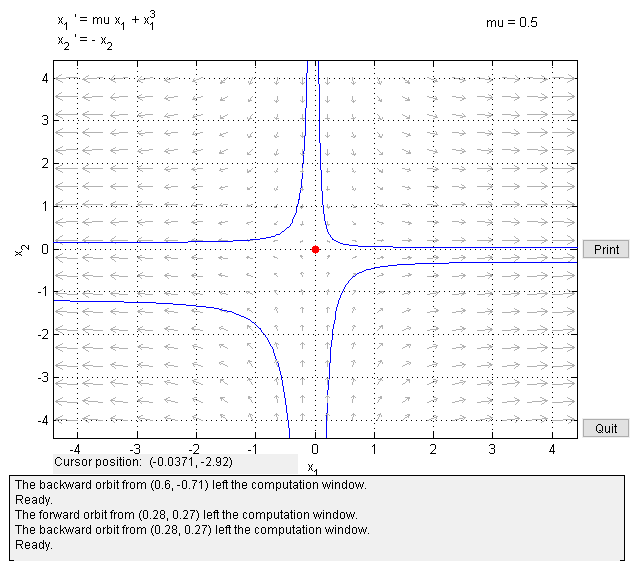
\includegraphics[width=\textwidth]{figures/lab2_4_pplane_pos.png}
	\caption{$\mu=0,5$}
    \end{subfigure}
    \caption{Espaço de estados do modelo do quarto sistema para diferentes parâmetros. Pontos de equilíbrio são representados por pontos vermelhos e as trajetórias dos estados são os traços azuis.}
    \label{fig:pplane-4}
\end{figure}

\end{document}
